\vspace{-8pt}
\section{Results and Analysis}
\label{sec:res}
\vspace{-5pt}
\subsection{Overall Performance}
\vspace{-3pt}
\label{sec:overall_perf}
\begin{table}[ht]
\centering
\scriptsize
\setlength{\tabcolsep}{2pt}
\vspace{-5pt}
\caption{Comparison of \hero with baselines. Best results are \textbf{bold}, second-best are \underline{underlined}. ``-'' indicates methods not designed for or evaluated on the task.} 
\label{tab:main_exp_res}
\vspace{-5pt}
\resizebox{\linewidth}{!}{
\begin{tabular}{l|ccc|ccc|ccc|ccc|ccc|c}
\toprule
\textbf{Dataset} 
& \multicolumn{3}{c|}{HotpotQA} 
& \multicolumn{3}{c|}{2WikiQA} 
& \multicolumn{3}{c|}{MusiQue} 
& \multicolumn{3}{c|}{AmbigQA} 
& \multicolumn{3}{c|}{Bamboogle} 
& HoVer \\
\cmidrule(r){2-4} \cmidrule(r){5-7} \cmidrule(r){8-10} 
\cmidrule(r){11-13} \cmidrule(r){14-16} \cmidrule(r){17-17}
\textbf{Metrics} 
& Acc & EM & F1 
& Acc & EM & F1 
& Acc & EM & F1 
& Acc & EM & F1 
& Acc & EM & F1 
& Acc \\
\midrule
\multicolumn{17}{l}{\textbf{\textit{Single-turn Retrieval}}} \\
\midrule
Qwen2.5-14B-Instruct & 43.53 & 35.72 & 46.14 & 26.64 & 26.25 & 31.85 & 9.23 & 7.00 & 13.75 & 39.78 & 36.65 & 50.23 & 27.20 & 34.70 & 34.35 & 45.50  \\
Qwen3-14B & 44.47 & 36.25 & 47.56 & 31.57 & 31.10 & 37.79 & 13.16 & 9.99 & 15.72 & 38.47 & 36.10 & 50.91 & 31.54 & 29.60 & 38.31 & 49.05 \\
Qwen3-8B & 41.35 & 33.70 & 45.10 & 26.37 & 26.10 & 32.12 & 11.49 & 8.71 & 13.62 & 36.02 & 33.80 & 47.70 & 23.87 & 22.40 & 30.28 & 50.15 \\
GPT-4o-mini & 46.30 & 37.74 & 49.30 & 28.42 & 28.41 & 35.11 & 16.63 & 13.94 & 19.60 & 37.40 & 33.80 & 47.99 & 38.36 & 36.00 & 42.81 & 47.95 \\
Llama3-3.1-8B-instruct & 33.16 & 27.02 & 35.14 & 20.40 & 20.35 & 25.11 & 8.43 & 6.43 & 12.61 & 18.03 & 18.96 & 24.60 & 20.46 & 19.20 & 27.24 & 49.90  \\
\midrule
\multicolumn{17}{l}{\textbf{\textit{Advanced RAG}}} \\
\midrule
Search-r1-7B & 51.11 & 41.94 & 54.18 & 48.89 & 44.69 & 49.20 & 20.45 & 18.58 & 25.73 & 47.32 & \underline{45.88} & \underline{65.54} & 35.79 & 32.64 & 43.93 & 47.76 \\
Iter-RetGen (Qwen2.5-7B) & 20.37 & 16.71 & 24.59 & 47.71 & 43.54 & 49.12 & 19.89 & 16.79 & 21.04 & --- & --- & --- & 35.33 & 34.12 & 40.65 & 51.29 \\
Plan-RAG 8b & 29.95 & 25.96 & 37.51 & 30.53 & 27.38 & 31.68 & 13.08 & 9.90 & 13.34 & --- & --- & --- & 30.01 & 23.57 & 32.12 & 50.33 \\
SELF-RAG (llama2-7B) & 23.85 & 13.64 & 25.07 & 40.82 & 37.30 & 42.02 & 8.47 & 7.16 & 14.16 & 28.51 & 24.03 & 39.62 & 25.80 & 22.66 & 30.05 & 40.52 \\
R1-Searcher 7B & 41.15 & 32.54 & 50.69 & 40.11 & 35.38 & 45.19 & 18.21 & 13.51 & 19.19 & --- & --- & --- & 41.00 & 38.85 & 46.76 & 51.56 \\
ExSearch (Qwen2.5-7B) & \underline{55.04} & 45.11 & 58.22 & 44.83 & 44.03 & 51.56 & 22.73 & 19.58 & 27.10 & -- & --- & -- & \textbf{56.12} & \textbf{51.27} & \textbf{63.80} & \underline{66.62} \\
DeepResearcher-7B & 40.65 & 35.23 & 58.86 & 49.40 & \underline{54.35} & \underline{64.05} & 24.53 & 18.56 & 25.57 & \underline{49.74} & 42.23 & 51.50 & 37.42 & 34.20 & 44.40 & 58.19 \\
IRCoT (GPT-4o-mini) & 40.39 & 33.14 & 54.93 & 38.73 & 35.50 & 42.01 & 19.11 & 18.23 & 25.00 & --- & --- & -- & 34.88 & 30.73 & 33.97 & 55.37 \\
InstructRAG-8B & 34.40 & 33.15 & 34.83 & 36.98 & 35.45 & 40.72 & 16.11 & 14.19 & 19.50 & 40.07 & 39.72 & 40.73 & 26.16 & 23.44 & 31.18 & 56.76 \\
CORAG-8B (Greedy) & 38.02 & 32.95 & 52.85 & 39.09 & 35.43 & 46.62 & 16.45 & 15.98 & 21.00 & 32.10 & 27.25 & 43.95 & 33.03 & 31.61 & 41.25 & 40.82\\
MMOA-RAG-8B & 30.02 & 26.02 & 34.75 & 35.56 & 31.89 & 38.58 & 16.47 & 13.36 & 18.82 & 38.85 & 34.75 & 48.59 & 34.47 & 31.76 & 42.01 & 58.19 \\
AceSearcher-8B & 42.91 & 37.19 & \textbf{68.07} & 50.83 & 45.59 & 52.75 & \underline{25.24} & 19.10 & 26.62 & -- & -- & -- & 47.21 & 45.12 & 51.91 & 59.37 \\
\midrule
\multicolumn{17}{l}{
\includegraphics[height=1em]{figures/hera.png} \textit{Ours} } \\
\midrule
\rowcolor{cyan!10} HERA (\qwen) & \textbf{55.38} & \textbf{52.50} & \underline{63.03} & \textbf{60.02} & \textbf{59.50} & \textbf{64.77} & \textbf{27.19} & \textbf{26.57} & \textbf{35.82} & \textbf{54.43} & \textbf{48.74} & \textbf{67.81} & \underline{49.01} & \underline{46.46} & \underline{60.53} & \textbf{67.35} \\
\rowcolor{cyan!10} HERA (\llama) & 53.28 & 48.01 & 57.91 & \underline{52.62} & 46.70 & 55.42 & 25.04 & \underline{24.46} & \underline{31.07} & 48.53 & 43.46 & 60.72 & 46.60 & 45.22 & 56.31 & 60.31 \\
\bottomrule
\end{tabular}}
\end{table}

\vspace{-8pt}

Table~\ref{tab:main_exp_res} compares \hero with a range of baselines (Direct inference and CoT results are reported in Appendix~\ref{app: ablte_llama}).  key observations are: \textbf{(i) Consistent gains over SOTA iterative and agentic RAG baselines}. \hero achieves an average of 38.69\% gains on all datasets compared against recent SOTA, demonstrating the effectiveness of experience-guided orchestration for interleaved reasoning and retrieval. Best AmbigQA performance highlights \hero’s robustness to queries with multiple plausible interpretations. \textbf{(ii) Robust OOD performance.} \hero ranks second on Bamboogle (F1 $-5.4\%$ vs. ExSearch) and first on HoVer ($+64.95\%$ vs. CORAG), reflecting the transferability of the accumulated experience library and evolving agent behaviors. In contrast, most prior approaches relying on heuristic planning or fixed iterative retrieval generalize poorly beyond in-distribution data. \textbf{(iii) Efficiency as gradient-free optimization}. \hero surpasses RL-fine-tuned multi-agent RAG methods, such as MMAO-RAG, showing that semantic group-wise advantages enable stable, consistent improvements across tasks and distribution shifts without costly model updates. \textbf{(iv) \hero-Qwen consistently outperforms \hero-Llama across all datasets}, particularly on cross-document reasoning and complex disambiguation tasks. While \hero-Llama remains competitive in-domain, its performance drops on OOD tasks, indicating limited reasoning and generalization capacity for ambiguous or sparse queries.


 

\vspace{-8pt}
\subsection{Ablation Study}
\label{sec:ablation}
\vspace{-5pt}
\begin{figure}[ht]
\vspace{-7pt}
        \centering
        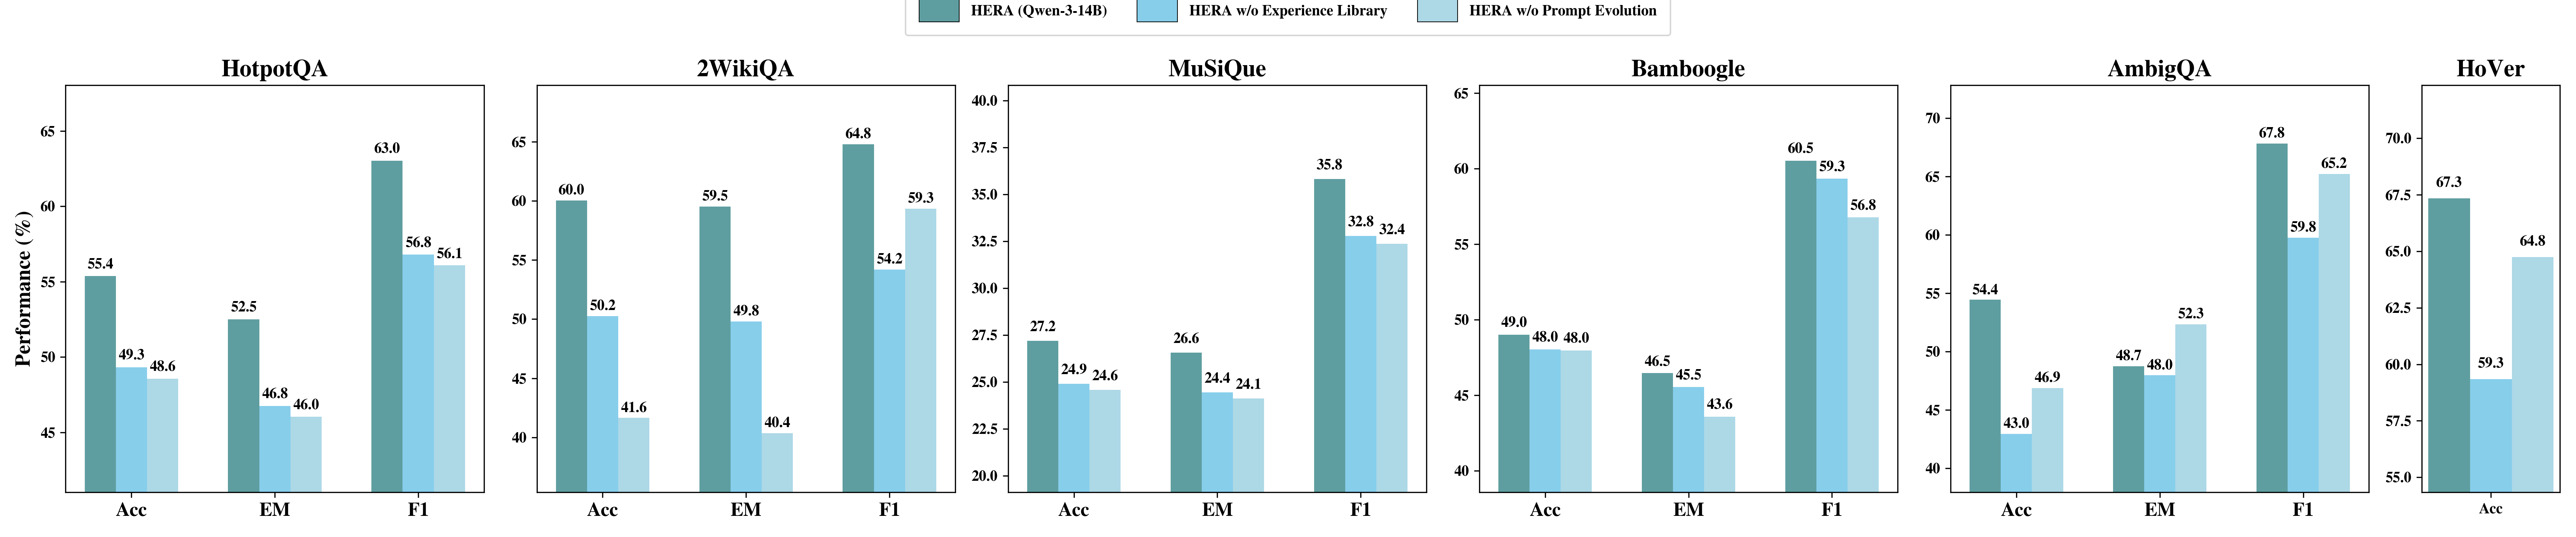
\includegraphics[width=1\linewidth]{figures/hera_per_dataset.png}
        \vspace{-8pt}
        \caption{Ablation Studies of \hero with \qwen as the backbone. }
        \label{fig:ablat_qwen}
        \vspace{-15pt}
    \end{figure}
 
Figure~\ref{fig:ablat_qwen} presents the ablation results of \hero on the test set using \qwen as the backbone (\llama results are provided in Appendix~\ref{app: ablte_llama}). Removing the experience library yields consistent but moderate performance declines across datasets (typically $\downarrow$ 6\% to 15\% relative accuracy), highlighting its role in improving knowledge guiding and cross-instance generalization. In contrast, omitting prompt evolution leads to substantially larger and more variable declines on multi-hop QA (up to $\downarrow$ 30\% relative on 2WikiQA for both backbones), where precise decomposition and trajectory control are essential. On ambiguity-intensive datasets AmbigQA, prompt evolution introduces a recall-oriented bias: improving F1 while occasionally reducing EM, whereas the experience library promotes precision through grounded outputs, revealing a systematic EM–F1 trade-off. These patterns are consistent across backbones, indicating that the functional contributions of each component are largely model-agnostic. Importantly, the full \hero framework consistently outperforms both ablations by a non-additive margin, indicating a positive interaction effect: improved reasoning behaviors from prompt evolution enhance the quality of stored experiences, which in turn reinforce subsequent reasoning through stronger grounding. Overall, the results demonstrate that prompt evolution and the experience library target complementary failure modes: procedural correctness versus epistemic reliability, and that their synergy is critical for robust multi-hop reasoning.
\vspace{-8pt}
\subsection{Performance-Efficiency Trade-off}
\label{sec:token_usage}
We examine the potential trade-off between performance and data efficiency by analyzing token usage patterns throughout learning. Our analysis emphasizes two key dimensions: (i) the dynamics of token consumption as learning progresses, and (ii) the interplay between token efficiency and task performance..

\label{sec:token_train}

\setlength{\intextsep}{-1pt}
\begin{wrapfigure}{r}{0.3\textwidth} % l = left, r = right
    \centering
    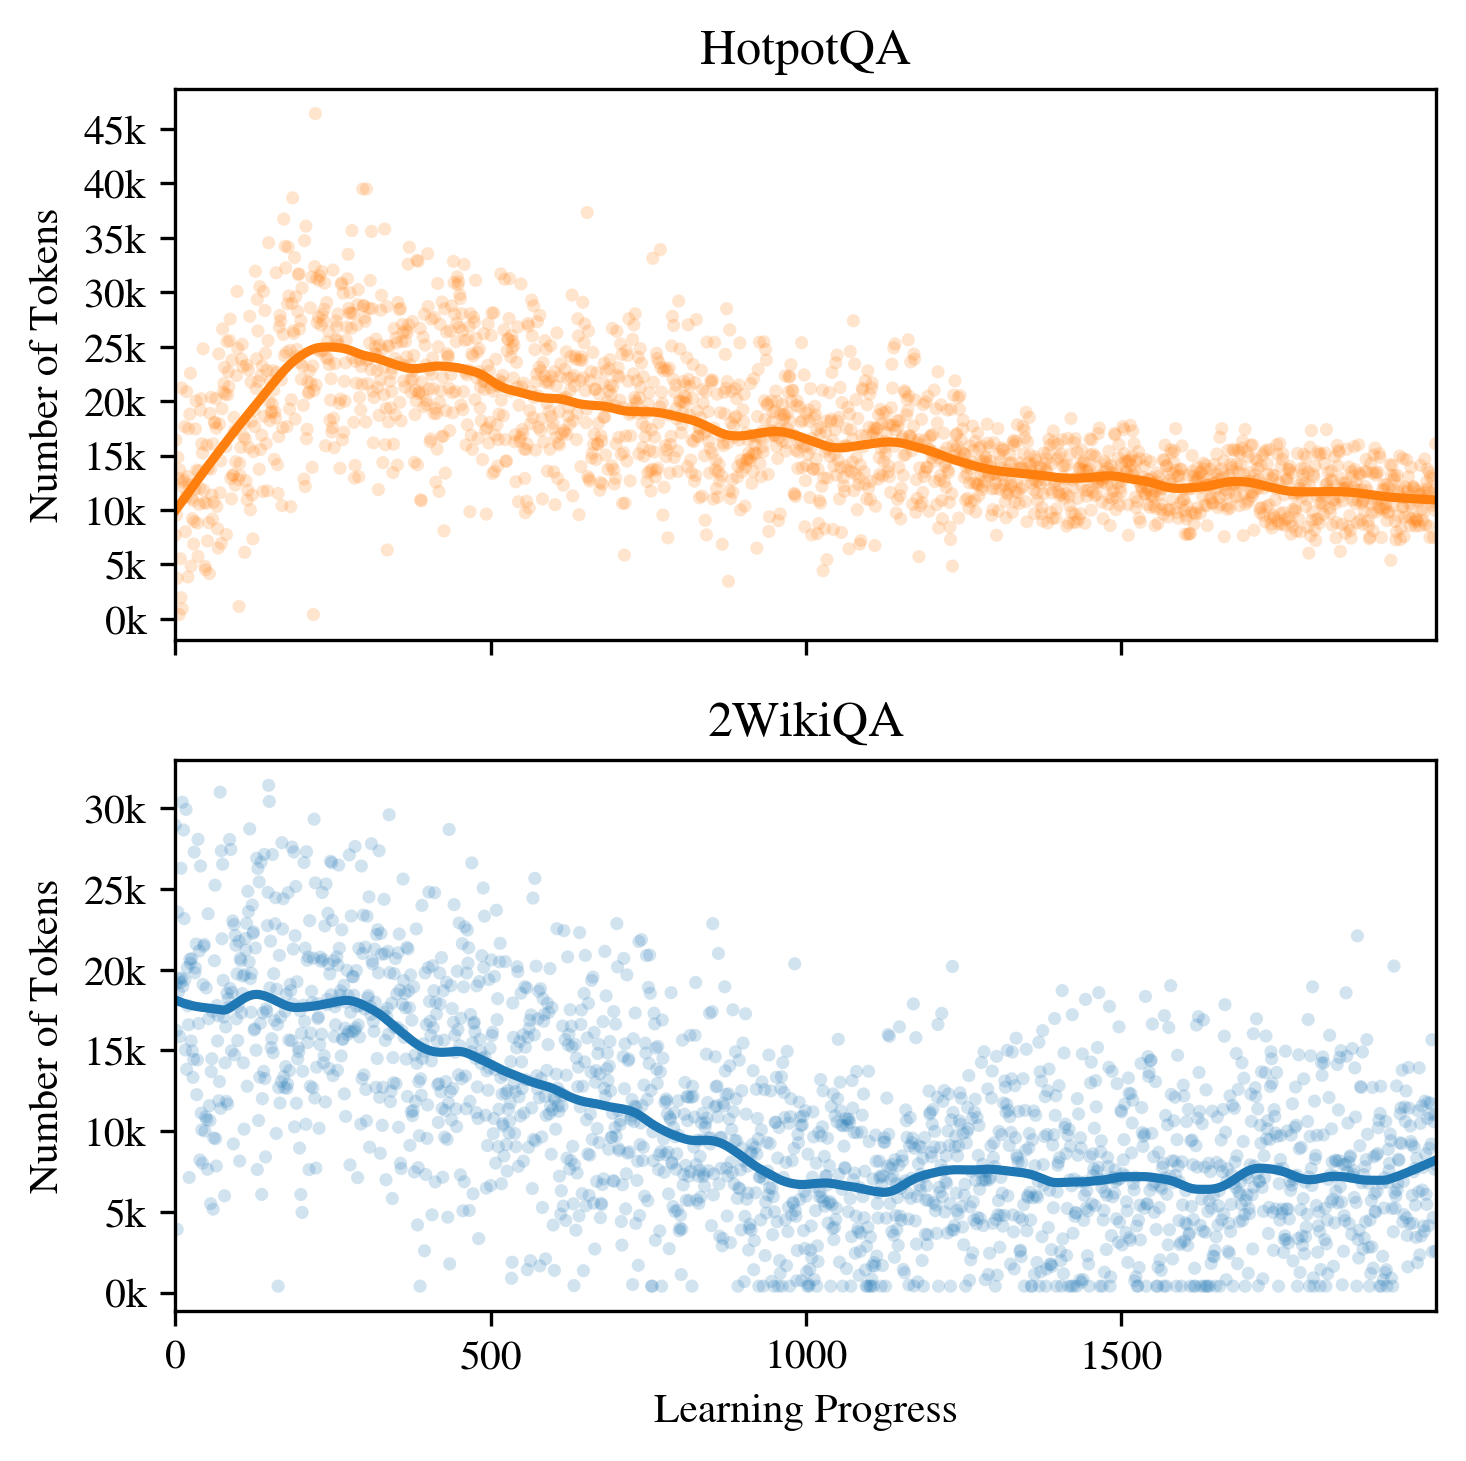
\includegraphics[width=\linewidth, height=3.6cm, keepaspectratio]{figures/HQA_Wiki__total_tokens.png}
    \caption{Token usage}
    \label{fig:lowess1}
\end{wrapfigure}
\vspace{-8pt}
\subsubsection{Dynamics of Token Consumption}
\vspace{-5pt}
\label{sec:token_train}
We visualize the token consumption throughout the learning process by Locally Weighted Scatterplot Smoothing (LOWESS) \citep{cleveland1981lowess, dang2025multi}. Figure~\ref{fig:lowess1} illustrates token usage trends on HotpotQA and 2WikiQA as representative tasks. \textbf{(i) Exploration–Exploitation Transition}. On HotpotQA, token consumption follows a non-monotonic trajectory. Early spikes reflect an exploratory phase in which the orchestrator activates multiple agents, constructs extended reasoning traces, and performs redundant steps to optimize performance. As experience accumulates, token usage declines monotonically, marking a transition to exploitation: low-efficiency agents are pruned, and reasoning chains are shortened. A subsequent plateau indicates convergence toward an efficient token budget. In contrast, 2WikiQA exhibits no initial exploratory peak, suggesting that transferable priors from previously accumulated reasoning experience support efficient agent orchestration with minimal trial-and-error. \textbf{(ii) Functional Contributions. } Token usage dynamics are tightly coupled with \hero’s experience library and prompt evolution. The library accumulates high-utility and generalizable experience, while evolving prompts enables agents to elevate their performance. Together, they drive emergent computational frugality, enabling high reasoning performance without explicit token-based penalties.
\vspace{-8pt}
\subsubsection{Performance vs.Token Usage}
\label{sec:performa_vs_token}
\begin{figure}[h]
        \centering
        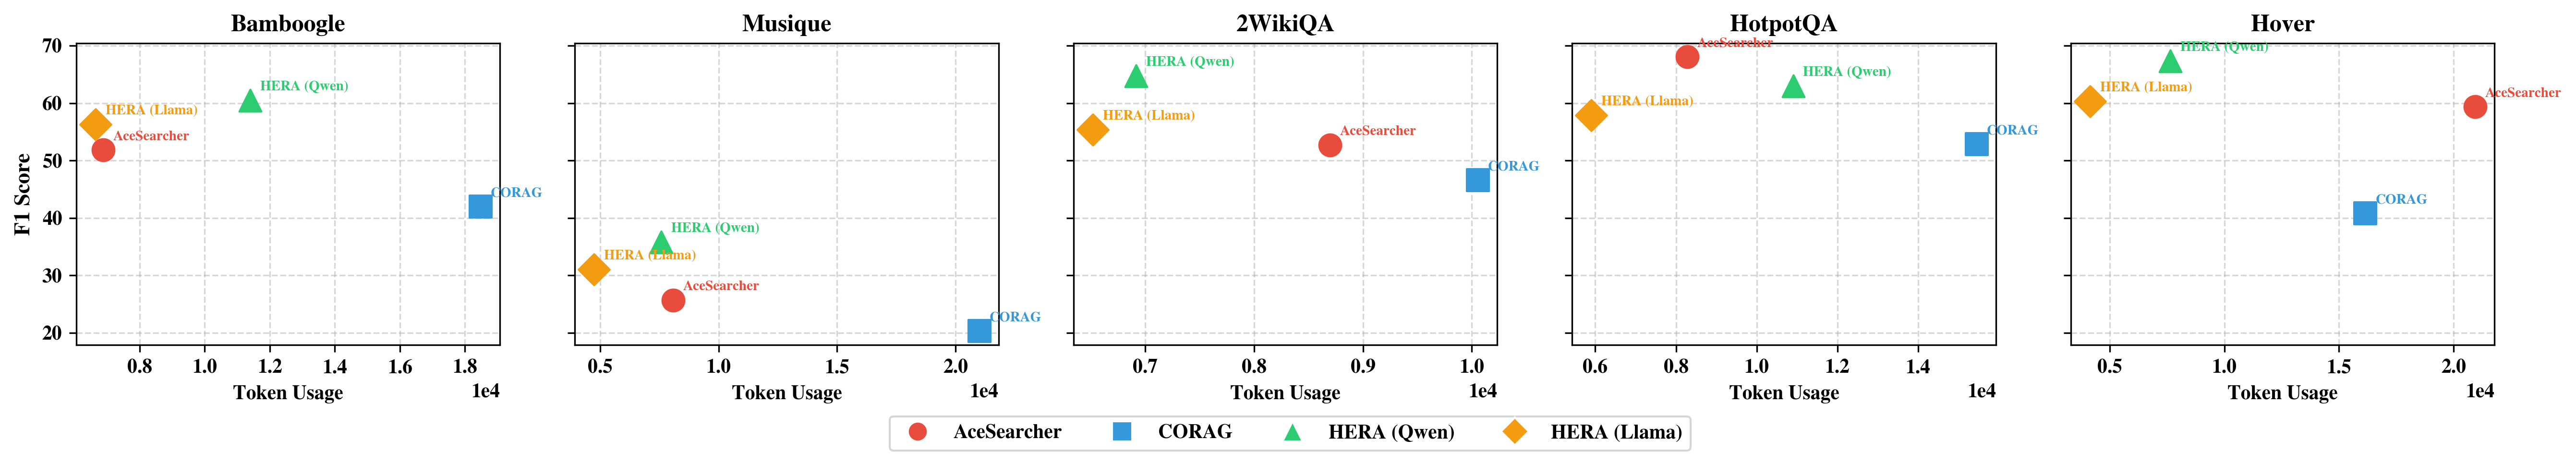
\includegraphics[width=1\linewidth]{figures/f1_vs_tokens.png}
        \vspace{-12pt}
        \caption{Comparison of Performance–Token Efficiency Trade-off with Selected Baselines.}
        \label{fig:f1_tokens}

    \end{figure}
\vspace{10pt}
Figure~\ref{fig:f1_tokens} compares multi-hop QA performance against token consumption. Key observations include: \textbf{(i) Superior Performance–Efficiency Trade-off}. Across all datasets, \hero consistently dominates the performance–efficiency frontier, achieving higher F1 scores with controlled token budgets. This demonstrates that gains arise from efficient reasoning trajectories instead of brute-force context scaling.
\textbf{(ii) Backbone-Specific Patterns.)} \hero with \qwen achieves the highest absolute performance, whereas \hero with \llama consistently minimizes token consumption ($\sim$4.7k–6.6k across most datasets) while preserving competitive F1 scores, indicating favorable computational efficiency. \textbf{(iii) Consistent performance and efficiency gains over baselines}.  CORAG uses the largest number of tokens across most datasets (up to $20k+$) without converting these costs into sustainable reasoning improvements or effective knowledge reuse, resulting in suboptimal F1 (\eg, 20.30 on MusiQue and 40.82 on HoVer). AceSearcher occupies an intermediate position, balancing moderate token usage and performance. 
\vspace{-8pt}
\subsection{Topology Evolution}
\vspace{-5pt}
\label{sec:topology_analysis}
To elucidate the emergence of coordinated multi-agent behavior, we systematically analyze the evolution of interaction topologies over the course of learning. For this purpose, we introduce topology-based metrics to quantify structural changes in agent collaboration.

\vspace{-5pt}
\subsubsection{Transition Entropy}
\label{sec:transition_entropy}
\begin{wrapfigure}{r}{0.32\textwidth}
    \vspace{-20pt} 
    \centering
    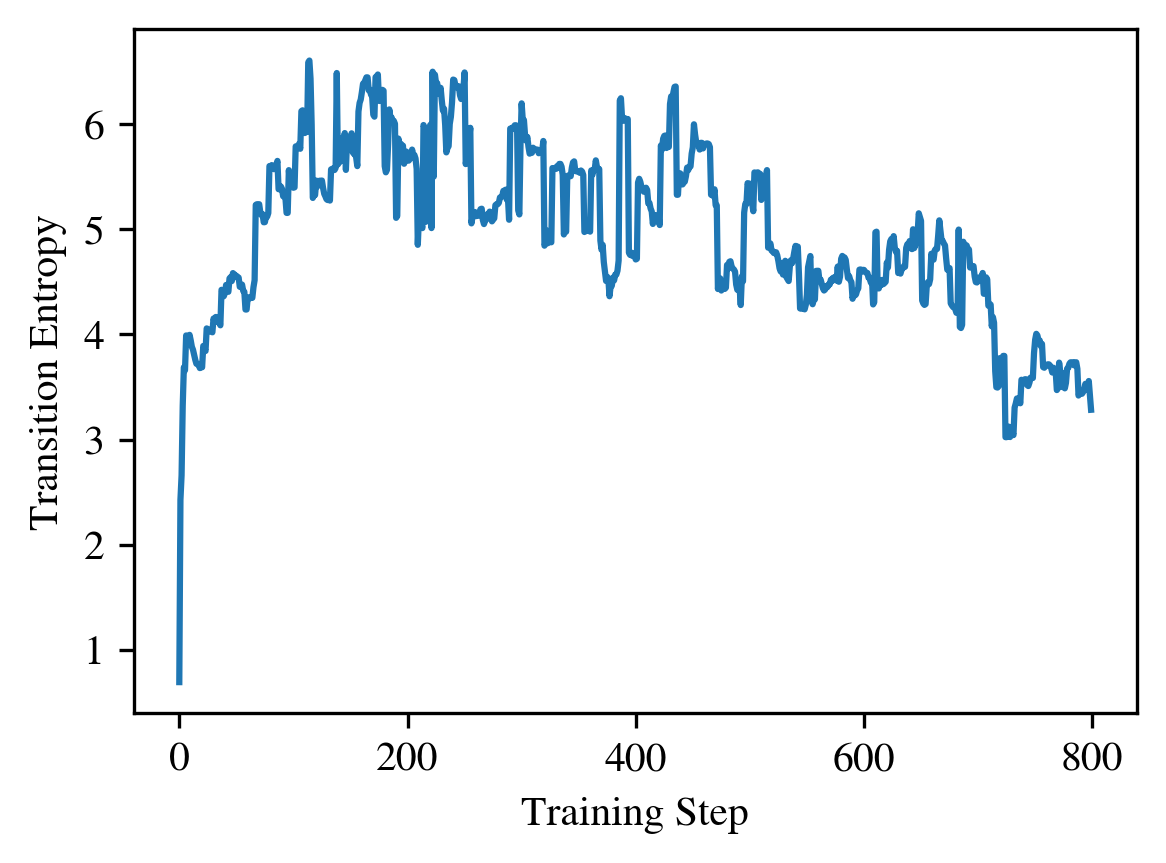
\includegraphics[width=\linewidth, height=3.3cm, keepaspectratio]{figures/transtion_ent.png}
    \vspace{-20pt} 
    \captionof{figure}{Transition entropy}
    \vspace{-20pt} 
        \label{fig:tran_entr}
        
\end{wrapfigure}
Transition Entropy quantifies the uncertainty in agent-to-agent transitions, capturing the policy-level dynamics. Let $Prob.(\mathcal{N}_{j}|\mathcal{N}_{i})$ denote the empirical transition probability from agent $\mathcal{N}_{i}$ to $\mathcal{N}_{j}$, the Transition Entropy is defined as:

\begin{flushleft}
\(
H_{trans} = -\sum_{i,j} Prob.(\mathcal{N}_{i} \to \mathcal{N}_{j})\,\log Prob.(\mathcal{N}_{i} \to \mathcal{N}_{j})
\)
\end{flushleft}
We compute $H_{trans}$ using a sliding-window over learning. Beyond the exploration–exploitation dynamics, Figure~\ref{fig:tran_entr} shows that after an initial rise, entropy stabilizes at an intermediate level, reflecting the emergence of structured yet flexible agent interactions. This plateau indicates that \hero consolidates high-value transition sequences while maintaining controlled exploration, enabling the system to integrate novel reasoning strategies without disrupting established coordination. The pattern highlights the complementary roles of the experience library, which reinforces effective multi-agent pathways, and prompt evolution, which adaptively refines agent behavior for functional alignment with task objectives. Notably, the plateau at intermediate entropy levels indicates controlled exploration even during exploitation, preventing premature convergence to suboptimal strategies while allowing the integration of novel cooperation pathways.

\vspace{-5pt}
\subsubsection{Graph-based Metrics}
\begin{wrapfigure}{r}{0.32\textwidth}

    \centering
    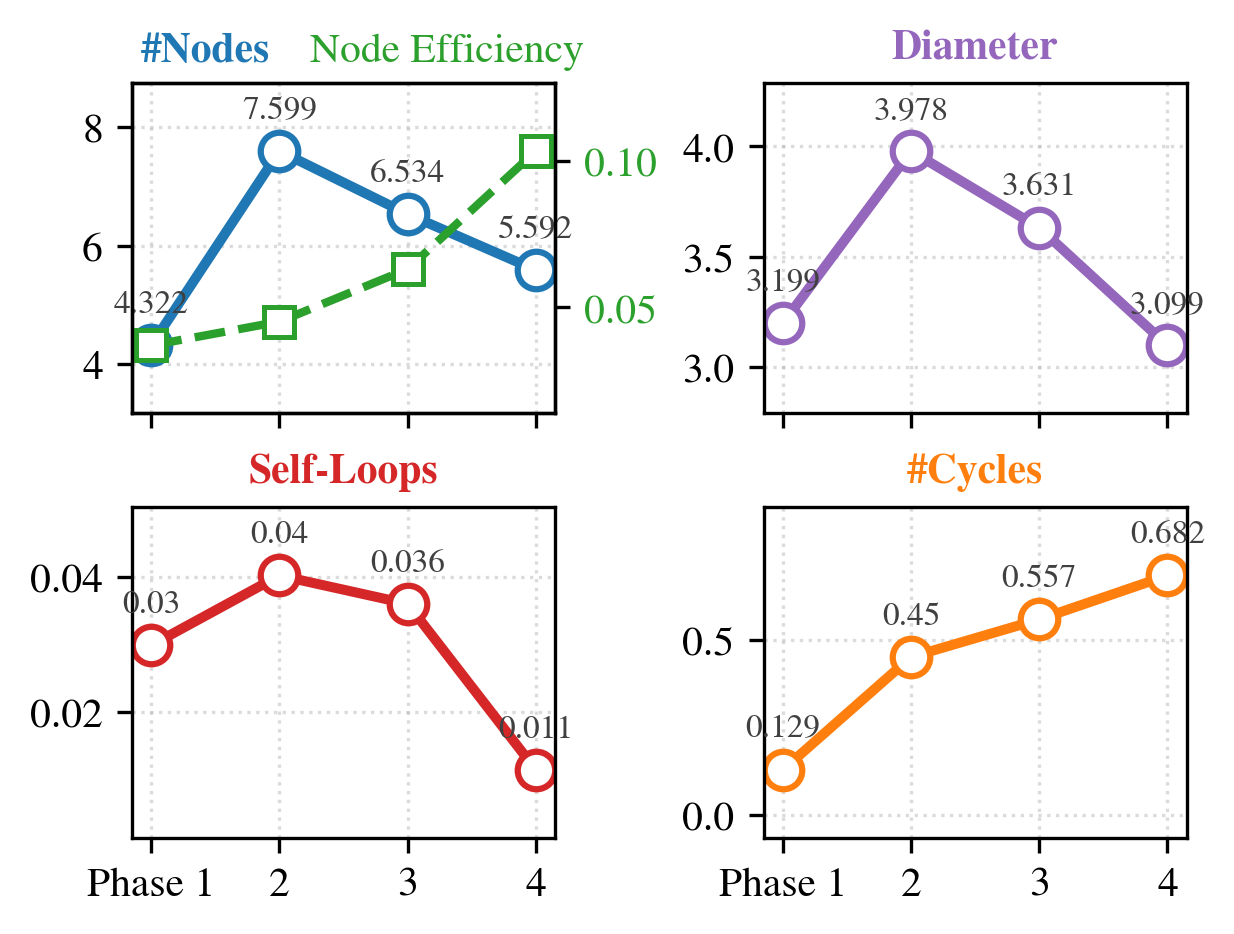
\includegraphics[width=\linewidth, height=3.3cm, keepaspectratio]{figures/nodesefficiency.png}
% 
    \captionof{figure}{Graph metrics}

    \label{fig:graph_metrics}
\end{wrapfigure} 
\vspace{-5pt}
To systematically characterize the topology evolution of \hero, we model each trajectory as a graph $\mathcal{G}_{\tau}=(V, E)$ where nodes represent agents and edges denote interactions. We quantify structural and functional properties via defining graph-theoretic metrics:
\textbf{(a) Number of agents $|V|$}: the total distinct agents involved in a trajectory, reflecting the breadth of collaboration.
\textbf{(b) Node efficiency}: per-agent contribution, formally by $\frac{\text{F1}(\tau)}{|V|}$, capturing per-agent utility.
\textbf{(c) Self-Loops}: the frequency of self-transitions, reflecting potential redundancy or degenerate reasoning.
\textbf{(d) Number of cycles}: count of closed-loop paths capturing iterative reasoning patterns.
\textbf{(e) Diameter}: longest shortest-path between any two nodes, representing maximum reasoning depth. 

We segment learning into four phases - initial, exploration, refinement, and optimization, and analyze normalized metrics per question type. As shown in Fig.~\ref{fig:graph_metrics}, Early trajectories are narrow and shallow, with low agent counts, minimal cycles, and limited diameter, reflecting sparse coordination. During exploration, the system dynamically recruits more agents, increasing diameter and cycle formation, capturing iterative reasoning and intermediate verification. By the refinement phase, trajectories contract: redundant agents and self-loops are pruned, diameter decreases, and node efficiency rises. This selective retention is guided by the experience library, which reinforces high-value interaction topologies, and by prompt evolution, which refines agent behaviors and intermediate outputs. The optimized phase exhibits compact chains with minimal nodes, high per-agent utility, and strategically preserved cycles, representing a balance of efficiency and robustness.

Overall, the evolving topologies reveal that \hero’s dual mechanisms - structured experience retrieval and adaptive prompt evolution enable a principled transition from exploratory, diffuse agent interactions to compact, high-utility, and resilient multi-agent system.





